\subsection{Åbne}

At ''åbne'' et billede betyder at vi bruger erosion først og dernæst dilation. Med dette vil følgende ske:

\begin{itemize}
	\item Udjævner konturerne.
	\item Deler objekter, som kun er forbundet med en tynd forbindelse.
	\item Fjerner tynde ''protrusions''.
\end{itemize}

Ligningen for at åbne et billede er vist på Figur~\ref{fig:openingeq}.

\begin{figure}[H]
	\centering
	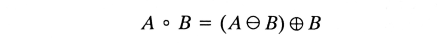
\includegraphics[width=0.5\linewidth]{figs/spm09/openingeq}
	\caption{Ligning for at ''åbne'' et billede.}
	\label{fig:openingeq}
\end{figure}

Figur~\ref{fig:opening-triangle} viser hvordan først erosion og så dilation på et billede foretages ved åbning. I den første trekant viser den prikkede linje hvordan erosionen påvirker billedet. Anden trekant viser kanten for den færdige åbning og den i den tredje er åbningen tydeligt farvet op.

\begin{figure}[H]
	\centering
	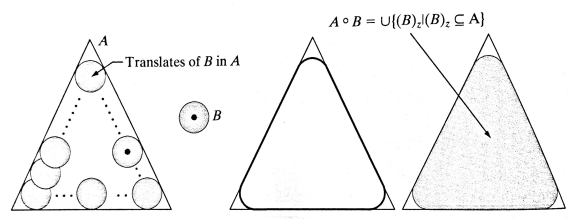
\includegraphics[width=0.9\linewidth]{figs/spm09/opening-triangle}
	\caption{Eksempel på at åbne et billede.}
	\label{fig:opening-triangle}
\end{figure}
